\documentclass{article}
\usepackage{tikz}
\usetikzlibrary{patterns}
\usetikzlibrary{patterns.meta}
% texdoc tikz, p 730

\begin{document}
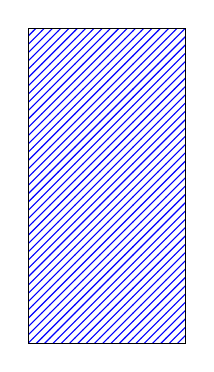
\begin{tikzpicture}
\draw[pattern=north east lines, pattern color=blue] (0,0) rectangle (2,4);
\end{tikzpicture}

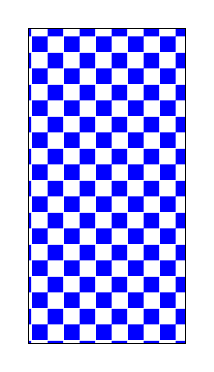
\begin{tikzpicture}
\draw[pattern=checkerboard, pattern color=blue] (0,0) rectangle (2,4);
\end{tikzpicture}

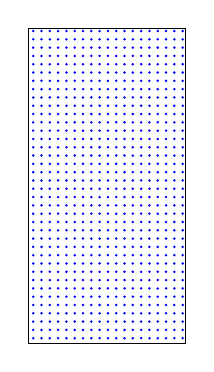
\begin{tikzpicture}
\draw[pattern=dots, pattern color=blue] (0,0) rectangle (2,4);
\end{tikzpicture}

\pgfdeclarepattern{
name=hatch,
parameters={\hatchsize,\hatchangle,\hatchlinewidth},
bottom left={\pgfpoint{-.1pt}{-.1pt}},
top right={\pgfpoint{\hatchsize+.1pt}{\hatchsize+.1pt}},
tile size={\pgfpoint{\hatchsize}{\hatchsize}},
tile transformation={\pgftransformrotate{\hatchangle}},
code={
\pgfsetlinewidth{\hatchlinewidth}
\pgfpathmoveto{\pgfpoint{-.1pt}{-.1pt}}
\pgfpathlineto{\pgfpoint{\hatchsize+.1pt}{\hatchsize+.1pt}}
\pgfpathmoveto{\pgfpoint{-.1pt}{\hatchsize+.1pt}}
\pgfpathlineto{\pgfpoint{\hatchsize+.1pt}{-.1pt}}
\pgfusepath{stroke}
}}


\tikzset{
hatch size/.store in=\hatchsize,
hatch angle/.store in=\hatchangle,
hatch line width/.store in=\hatchlinewidth,
hatch size=5pt,
hatch angle=0pt,
hatch line width=.5pt,
}


\begin{tikzpicture}
\draw[pattern=hatch, pattern color=red] (0,0) rectangle (2,4);
\end{tikzpicture}

\begin{tikzpicture}
\foreach \r in {1,...,4}
\draw [pattern=hatch, pattern color=red]
(\r*3,0) rectangle ++(2,2);
\foreach \r in {1,...,4}
\draw [pattern=hatch, pattern color=green, hatch size=2pt]
(\r*3,3) rectangle ++(2,2);
\foreach \r in {1,...,4}
\draw [pattern=hatch, pattern color=blue, hatch size=10pt, hatch angle=21]
(\r*3,6) rectangle ++(2,2);
\foreach \r in {1,...,4}
\draw [pattern=hatch, pattern color=orange, hatch line width=2pt]
(\r*3,9) rectangle ++(2,2);
\end{tikzpicture}


\end{document}